\themaN
\graphicspath{{../../S29_Introduction_aux_equations/Images/}}

\chapter{Introduction\\aux équations}
\label{S29}


%%%%%%%%%%%%%%%%%%%%%%%%%%%%%%%%%%%%
%%%%%%%%%%%%%%%%%%%%%%%%%%%%%%%%%%%%
\begin{prerequis}
   \begin{itemize}
      \item Notion d'inconnue, d'équation.
      \item[\com] Utiliser le calcul littéral pour valider ou réfuter une conjecture, pour modéliser une situation.
   \end{itemize}
\end{prerequis}

\vfill

\begin{debat}[Débat : les équations]
   Aussi loin que remontent les textes connus en mathématiques, on y trouve des questions que l'on modéliserait aujourd'hui par des {\bf équations} qui consistent à remplacer les valeurs inconnues par des lettres (souvent $x$) et à exprimer un lien entre les inconnues et des grandeurs caractérisées par des nombres. L'objectif est de trouver la ou les inconnues, sachant qu'il n'est pas toujours possible de les déterminer algébriquement.
   \begin{center}
      \begin{pspicture}(-1,0)(5,3.5)
         \textcolor{B1}{
         \rput{10}(1,1){$x+5=0$}
         \rput{-15}(2,3){$x^2-5x+4=0$}
         \rput{5}(3,2){$\text{e}^x-4=0$}
         \rput{-15}(0,2){$3x-6=0$}
         \rput{-20}(3.75,0.75){$2\sqrt{x}=4$}}
      \end{pspicture}
   \end{center}
   \begin{cadre}[B2][F4]
      \begin{center}
         Vidéo : \href{https://leblob.fr/fondamental/les-equations}{\bf Les équations}, site Internet {\it Le blob}, épisode de la série {\it Petits contes mathématiques}.
      \end{center}
   \end{cadre}
\end{debat}

\vfill

\textcolor{PartieGeometrie}{\sffamily\bfseries Cahier de compétences} : chapitre 4, exercices 23 à 36 ; 40 à 42.


%%%%%%%%%%%%%%%%%%%%%%%%%%%%%%%%%
%%%%%%%%%%%%%%%%%%%%%%%%%%%%%%%%%
\activites

\begin{activite}[Programme de calcul]
   {\bf Objectifs :} tester une égalité ; utiliser un tableau numérique (tableur) ; établir une expression littérale.
   \begin{QCM}
      On considère le programme de calcul suivant. À l'issue de ce programme, on obtient 257.
      \begin{center}
         \shadowbox{\begin{minipage}{7cm}
            Choisir un nombre. \\
            Lui ajouter 3. \\
            Multiplier le résultat par 5. \\
            Ajouter le double du nombre choisi au départ.
         \end{minipage}}
      \end{center}
      
      \partie[tester des valeurs à la main]
      \ \\ [-10mm]
         \begin{enumerate}
            \item Tester le programme avec 0 : \pfb \smallskip
            \item Tester le programme avec 1 : \pfb \smallskip
            \item Tester le programme avec 10 : \pfb \smallskip
            \item Tester le programme avec 22 : \pfb \bigskip
         \end{enumerate}

      \partie[tester des valeurs à l'aide d'un tableur] %%%%%
         On s'aperçoit très vite que pour trouver la valeur de départ, il faut procéder à de nombreux essais à moins de tomber \og par hasard \fg{} sur la bonne valeur. On ne peut pas non plus \og remonter \fg{} l'algorithme car dès le début, il faudrait connaître la valeur de départ. Afin de limiter les calculs, on va donc s'aider d'un tableur. \\
         \newcolumntype{M}{>{\itshape\footnotesize}p{4cm}}
         {\hautab{1.4}
         \begin{tabular}{C{0.1}p{11cm}C{0.1}M}
            \textcolor{B1}{\bf 5)}
            &
            Ouvrir un tableur présent sur l'ordinateur.
            & & \\
            \textcolor{B1}{\bf 6)}
            &
            \multicolumn{3}{p{15cm}}{Remplir la première ligne ainsi : \newline
            \footnotesize
            \begin{tabular}{|>{\columncolor{lightgray!30}}c|p{2cm}|p{1.5cm}|p{4cm}|p{5cm}|}
               \hline
               \rowcolor{lightgray!30} & \centering A & \centering B &  \centering C & \hspace*{2.75cm} D \\
               \hline
               1 & nombre choisi & ajouter 3 & multiplier le résultat par 5 & ajouter le double du nombre de départ \\
               \hline
            \end{tabular}} \\
            \textcolor{B1}{\bf 7)}
            &
            Dans la cellule \fbox{\texttt{A2}}, inscrire 0. \newline
            Dans la cellule \fbox{\texttt{B2}}, écrire la formule suivante : \, \fbox{\texttt{=A2}+3} \newline
            Que signifie cette formule ? Quel résultat s'affiche dans cette cellule ? \newline
            \pf
            & &
            \ding{43} Une cellule est désignée par un couple lettre-nombre qui indique la case à l'intersection de la colonne lettre et de la ligne nombre. \\          
            \textcolor{B1}{\bf 9)}
            &
            Quelle formule doit-on entrer dans la cellule \fbox{\texttt{C2}} pour obtenir le résultat de la cellule \fbox{\texttt{B2}} multiplié par 5 ? Vérifier que le résultat affiché est cohérent. \newline
            \pf
            & & 
            \ding{43} Pour saisir une formule dans une cellule, il faut commencer par le signe \fbox{\texttt{$=$}} pour indiquer qu'il s'agit d'un calcul. \\
             \textcolor{B1}{\bf 10)}
            &
            Quelle formule doit-on entrer dans la cellule \fbox{\texttt{D2}} pour obtenir le résultat de la somme de la cellule de la cellule \fbox{\texttt{C2}} et du double du nombre de départ ? Vérifier que le résultat affiché est cohérent. \pfb
            & &
            \ding{43} Dans une feuille de calcul, le signe de multiplication est l'étoile \fbox{*} \\
            \textcolor{B1}{\bf 11)}
            &
            Afin de tester un grand nombre de valeurs, on entre les nombres de 0 à 50 dans la colonne \fbox{\texttt{A}} : entrer dans la cellule \fbox{\texttt{A3}} le nombre 1, sélectionner les cellules \fbox{\texttt{A2}} et \fbox{\texttt{A3}} puis copier la sélection vers le bas jusqu'à 50.
            & &
            \ding{43} Pour copier les cellules, sélectionner le coin inférieur droit des deux cellules sélectionnées puis glisser la souris vers le bas. \\
            \textcolor{B1}{\bf 12)}
            &
            Sélectionner les cellules \fbox{\texttt{B2}} à \fbox{\texttt{D2}} et les copier vers le bas.
            & & \\
            \textcolor{B1}{\bf 14)}
            &
            Conclure sur la solution du problème.
            \pf
            & & \\ [6mm]
         \end{tabular}}
   \end{QCM} 
\end{activite}


%%%%%%%%%%%%%%%%%%%%%%%%%%%%%%%%%%%%
%%%%%%%%%%%%%%%%%%%%%%%%%%%%%%%%%%%%
\cours 

\section{Notion d'équations} %%%%%
  
\begin{definition}
   \begin{itemize}
      \item Une {\bf équation} est une égalité entre deux expressions où apparaissent des {\bf inconnues} désignées par des lettres. 
      \item {\bf Résoudre} l’équation, c’est trouver toutes les valeurs possibles pour l’inconnue. \\
      Ces valeurs sont appelées des {\bf solutions} de l'équation.
   \end{itemize}
\end{definition}

\begin{pspicture}(-2,0.5)(10.5,3.8)
  \rput(4,2){\LARGE \textcolor{A1}{$2x+5$} $=$ \textcolor{B1}{105}}
  \psbrace[nodesepA=-9mm,nodesepB=3mm,rot=90](2.3,1.7)(4,1.7){\textcolor{A1}{1\up{er} membre}}
  \psbrace[nodesepA=-8mm,nodesepB=3mm,rot=90](4.6,1.7)(5.8,1.7){\textcolor{B1}{2\up{e} membre}}
  \rput(2.9,3.1){inconnue $x$}
  \psline{<-}(2.83,2.3)(2.83,2.8)
  \rput(9,1.6){\parbox{3cm}{\it La solution de cette équation est le nombre réel $x =50$}}
\end{pspicture}


%%%%%%%%%%%%%%%%%%%%%%%%%%%%%%%%%%%%
\section{Tester une égalité}

\medskip

\begin{methode*2*2}[Résoudre une équation en testant une égalité]
    Pour résoudre une équation, on peut tester différentes valeurs de l'inconnue et vérifier que les deux membres de l'égalité sont égaux en effectuant les étapes suivantes :
   \begin{enumerate}
      \item on écrit séparément les deux membres de l'égalité ;
      \item on remplace l'inconnue par la valeur numérique dans chaque membre ;
      \item on calcule la valeur de chaque membre :
      \begin{itemize}
         \item si elles sont égales, l'égalité est vraie.
         \item si elles ne sont pas égales, l'égalité est fausse.
      \end{itemize}
   \end{enumerate}
   \exercice
      L'égalité $2x+1 =5x-5$ est-elle vraie pour $x =3$ ?
   \correction
      Pour $x =3$, on a :
      \begin{itemize}
         \item $2x+1 =2\times3+1 =7.$
         \item $5x-5 =5\times3-5 =10.$
      \end{itemize}
      Les deux membres de l'égalité ne sont pas égaux, donc l'égalité n'est pas vraie pour $x=3$.
   \exercice
      L'égalité $2x+1 =5x-5$ est-elle vraie pour $x =2$ ?
   \correction
      Pour $x =2$, on a :
      \begin{itemize}
         \item $2x+1 =2\times2+1 =5$.
         \item $5x-5 =5\times2-5 =5$.
      \end{itemize}
      Les deux membres de l'égalité sont égaux, donc l'égalité est vraie pour $x=2$. \\
      On dit que 2 est une solution de l'équation \\
      $2x+1 =5x-5$.
\end{methode*2*2}

\bigskip

\begin{remarque}
   en cinquième, on résout une équation en testant des valeurs pour l'inconnue. La résolution algébrique sera abordée à partir de la quatrième.
\end{remarque}

%%%%%%%%%%%%%%%%%%%%%%%%%%%%%%%%%%%%
%%%%%%%%%%%%%%%%%%%%%%%%%%%%%%%%%%%%
\exercicesbase

\begin{colonne*exercice}

\serie{Tester une égalité} %%%%%

\bigskip

\begin{exercice} %1
   L'égalité $5x =2x+15$ est-elle vérifiée :
   \begin{enumerate}
      \item Pour $x =4$.
      \item Pour $x =5$.
   \end{enumerate}
\end{exercice}

\begin{corrige}
   \ \\ [-5mm]
   \begin{enumerate}
      \item $5x =5\times4 =20$ et $2x+15 =2\times4+15 =23$. \\
       donc, pour $x =4$, {\blue l'égalité n'est pas vérifiée}.
      \item $5x =5\times5 =25$ et $2x+15=2\times5+15 =25$. \\
       donc, pour $x =5$, {\blue l'égalité est vérifiée.}
   \end{enumerate}
\end{corrige}

\bigskip


\begin{exercice} %2
   \begin{enumerate}
      \item Montrer que pour $x =3$, l'égalité $2x^2 =6x$ est vérifiée.
      \item Peut-on trouver un autre nombre pour lequel l'égalité précédente est vérifiée ?
   \end{enumerate}
\end{exercice}

\begin{corrige}
   \ \\ [-5mm]
   \begin{enumerate}
      \item $2x^2 =2\times3^2 =18$ et $6x =6\times3 =18$. \\
      donc, pour $x =3$, {\blue l'égalité est vérifiée}.
      \item $2x^2 =2\times0^2 =0$ et $6x =6\times0 =0$. \\
      donc, {\blue pour $x =0$} l'égalité est encore vérifiée.
   \end{enumerate}
\end{corrige}

\bigskip


\begin{exercice} %3
   Déterminer si l'égalité $3y =4x-3$ est vérifiée :
   \begin{enumerate}
      \item pour $y =3$ et $x =3$.
      \item pour $y =2$ et $x =4$.
   \end{enumerate}
\end{exercice}

\begin{corrige}
   \ \\ [-5mm]
   \begin{enumerate}
      \item $3y =3\times3 =9$ et $4x-3 =4\times3-3 =9$. \\
      donc, pour $y =3$ et $x =3$, {\blue l'égalité est vérifiée}.
      \item $3y =3\times2 =6$ et $4x-3 =4\times4-3 =13$. \\
      donc, pour $y =2$ et $x =4$, {\blue l'égalité n'est pas vérifiée}.
   \end{enumerate}
\end{corrige}

\bigskip


\serie{Résoudre une équation} %%%%%

\bigskip

\begin{exercice} %4
   Compléter les opérations à trou suivantes. \smallskip
   \begin{colenumerate}{2}
      \item $4\times\pfb =8$ \hfill \smallskip
      \item $6\times\pfb =54$ \hfill \smallskip
      \item $\pfb\times25 =50$ \hfill \smallskip
      \item $1\times\pfb =89$ \hfill \smallskip
      \item $\pfb\times21=0$ \hfill \smallskip
      \item $10\times\pfb =10$ \hfill
      \item $4\times\pfb =2$ \hfill
      \item $\pfb\times4 =6$ \hfill
      \item $5\times\pfb =22$ \hfill
      \item \, $4\times\pfb =3$ \hfill
   \end{colenumerate}
\end{exercice}

\begin{corrige}
   \ \\ [-5mm]
   \begin{colenumerate}{2}
      \item $4\times{\blue 2} =8$
      \item $6\times{\blue 9} =54$
      \item ${\blue 2}\times25 =50$
      \item $1\times{\blue 89} =89$
      \item ${\blue 0}\times21=0$
      \item $10\times{\blue 1} =10$
      \item $4\times{\blue 0,5} =2$
      \item ${\blue 1,5}\times4 =6$
      \item $5\times{\blue 4,4} =22$
      \item \, $4\times{\blue 0,75} =3$
   \end{colenumerate}
\end{corrige}

\bigskip


\begin{exercice} %5
   Compléter les opérations à trou suivantes. \smallskip
   \begin{colenumerate}{2}
      \item $2+\pfb =16$ \hfill \smallskip
      \item $5+\pfb =15$ \hfill \smallskip
      \item $18+\pfb =0$ \hfill \smallskip
      \item $18+\pfb =8$ \hfill \smallskip
      \item $-3+\pfb =1$ \hfill \smallskip
      \item $-5+\pfb =-7$ \hfill
      \item $+2+\pfb =6$ \hfill
      \item $-7+\pfb =-3$ \hfill
      \item $+6+\pfb =3$ \hfill
      \item \, $10+\pfb =-4$ \hfill
   \end{colenumerate}
\end{exercice}

\begin{corrige}
   \ \\ [-5mm]
   \begin{colenumerate}{2}
      \item $2+{\blue 14} =16$
      \item $5+{\blue 10} =15$
      \item $18+{\blue (-18)} =0$
      \item $18+{\blue (-10)} =8$
      \item $-3+{\blue 4} =1$
      \item $-5+{\blue (-2)} =-7$
      \item $+2+{\blue 4} =6$
      \item $-7+{\blue 4} =-3$
      \item $+6+{\blue (-3)} =3$
      \item \, $10+{\blue (-14)} =-4$
   \end{colenumerate}
\end{corrige}

\bigskip


\begin{exercice} %6
   Résoudre de tête les équations suivantes. \smallskip
   \begin{colenumerate}{2}
      \item $3+x =25$ \smallskip
      \item $-15+x =32$ \smallskip
      \item $2+x =-5,8$ \smallskip
      \item $-45+x =-47$ \smallskip
      \item $x+42 =78$ \smallskip
      \item $x-28 =14$
      \item $x+48 =-29$
      \item $x-8,5 =7$
      \item $3\times m =15$
      \item \, $t\times5 =3,5$
   \end{colenumerate}
\end{exercice}

\begin{corrige}
   \ \\ [-5mm]
   \begin{colenumerate}{2}
      \item $x =25-3 =\blue 22$
      \item $x =32+15 =\blue 47$
      \item $x =-5,8-2 =\blue -7,8$
      \item $x =-47+45 =\blue -2$
      \item $x =78-42 =\blue 36$
      \item $x =14+28 =\blue 42$
      \item $x=-29-48 =\blue -77$
      \item $x=7+8,5 =\blue 15,5$
      \item $m =15\div3 =\blue 5$
      \item \, $t =3,5\div5 =\blue 0,7$
   \end{colenumerate}
\end{corrige}

\bigskip


\serie{Petits défis} %%%%%

\bigskip

\begin{exercice} %7
   Adam a inscrit un nombre sur sa calculatrice puis a
tapé la suite de touches suivantes :
   \begin{center}
      \fbox{\large$\times$} \quad \fbox{\large5} \quad \fbox{\large$+$} \quad \fbox{\large8}
   \end{center}
   \begin{enumerate}
      \item Combien a-t-il trouvé en ayant choisi le nombre 24 ?
      \item Adam a trouvé 43, quel nombre avait-il écrit sur sa calculatrice ?
      \item Il se demande quel nombre afficher pour obtenir 12. Pouvez-vous l'aider ?
   \end{enumerate}
\end{exercice}

\begin{corrige}
   \ \\ [-5mm]
   \begin{enumerate}
      \item Avec 24, on obtient la suite : $24 \xrightarrow{\times5} 120 \xrightarrow{+8} \blue 128$ \smallskip
      \item Pour obtenir 43, on effectue les opération inverses : $43 \xrightarrow{-8} 35 \xrightarrow{\div5} {\blue 7}$ \smallskip
      \item Pour obtenir 12, on effectue les opération inverses : $12 \xrightarrow{-8} 4 \xrightarrow{\div5} {\blue 0,8}$
   \end{enumerate}
\end{corrige}

\medskip


\begin{exercice} %8
   Voici un programme :
   \begin{center}
      \fbox{\begin{minipage}{4cm}
         {\it Choisi un nombre. \\
         Retire-lui 3. \\
         Multiplie le résultat par 5.}
      \end{minipage}}
   \end{center}
   \begin{enumerate}
      \item Faire fonctionner le programme avec trois nombres de votre choix supérieurs à 3.
      \item Quel nombre faut-il choisir pour obtenir 15 ?
      \item Quel nombre faut-il choisir pour obtenir 0 ?
      \item Soit $x$ le nombre de départ, donner l'expression finale en fonction de $x$.
   \end{enumerate}
\end{exercice}

\begin{corrige}
   \ \\ [-5mm]
   \begin{enumerate}
      \item Avec 4, on obtient la suite : $4 \xrightarrow{-3} 1 \xrightarrow{\times5} \blue 5$ \\ \smallskip
         Avec 9, on obtient la suite : $9 \xrightarrow{-3} 6 \xrightarrow{\times5} \blue 30$ \\ \smallskip
         Avec $100$, on obtient la suite : $100 \xrightarrow{-3} 97 \xrightarrow{\times5} \blue 485$ \smallskip
      \item Pour avoir 15, on doit choisir 6 : $15 \xrightarrow{\div5} 3 \xrightarrow{+3} \blue 6$
      \item Pour avoir 0, on doit choisir 3 : $0 \xrightarrow{\div5} 0 \xrightarrow{+3} \blue 3$
      \item Avec $x$, on a : $x \xrightarrow{-3} x-3 \xrightarrow{\times5} 5(x-3) ={\blue 5x-15}$ \\
   \end{enumerate}
\end{corrige}

\medskip


\begin{exercice} %9
   La somme de trois entiers consécutifs est 72. \\
   Quels sont ces nombres ? \\
\end{exercice}

\begin{corrige}
   On peut tester avec différents nombres jusqu'à obtenir le résultat. On peut aussi diviser 72 par 3, on obtient 24. 24 est la moyenne des trois nombres, donc {\blue les trois nombres sont 23, 24 et 25}  \\ [2mm]
   Méthode algébrique : soit $x$ le premier nombre entier, le second est $x+1$ et le troisième $x+2$. \\
   La somme des nombres vaut $x+(x+1)+(x+2) =3x+3$. \\
   On résout donc l'équation $3x+3 =72$\dots
\end{corrige}

\bigskip


\begin{exercice} %10
   Smaïl est allé au marché et avec \ueuro{14,53} il a
acheté :
   \begin{itemize}
      \item \ukg{1,1} de viande à \ueuro{10,50} le kilogramme ;
      \item \ug{250} d'olives à \ueuro{8,52} le kilogramme ;
      \item un melon.
   \end{itemize}
   \begin{center}
      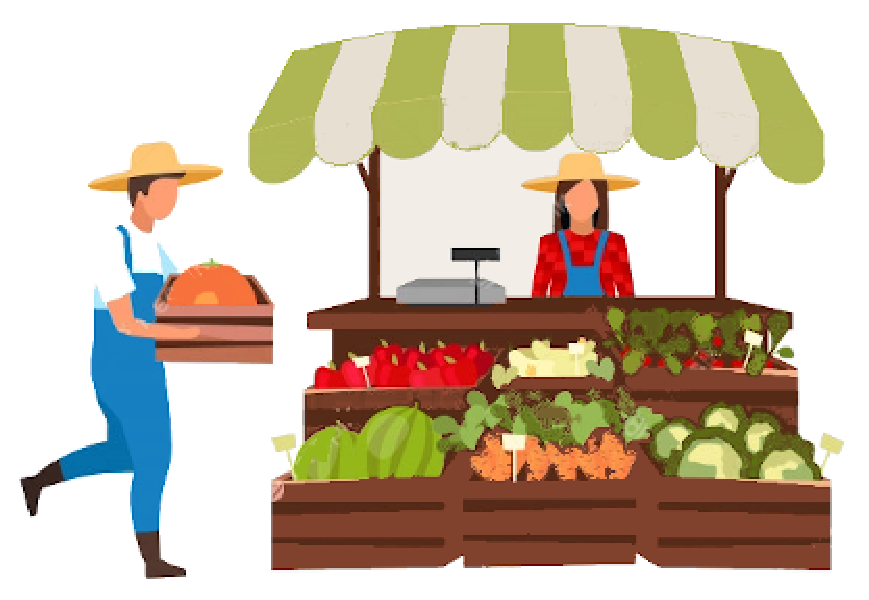
\includegraphics[width=3.5cm]{Marche}
   \end{center}
   \begin{enumerate}
      \item Quel est le prix du melon ?
      \item On note $m$ le prix de melon, quelle équation permet de résoudre le problème de manière littérale ?
   \end{enumerate}
\end{exercice}

\begin{corrige}
  \ \\ [-5mm]
   \begin{enumerate}
      \item Smaïl a payé : \\
      $1,1\times\ueuro{10,50}=\ueuro{11,55}$ pour la viande ; \\
      $0,25\times\ueuro{8,52} =\ueuro{2,13}$ pour les olives ; \\
      au total, cela fait $\ueuro{11,55}+\ueuro{2,13} =\ueuro{13,68}$ pour ces deux articles pour un total de \ueuro{14,53}. \\
      Il reste donc $\ueuro{14,53}-\ueuro{13,68} =\blue \ueuro{0,85}$ pour le melon.
      \item On a : $1,1\times10,50+0,25\times8,52+m =14,53$ \\
       Soit : $\blue 3,68+m =14,53$
   \end{enumerate}
   
\bigskip
\corec{En route pour la quatrième}
\medskip

\begin{enumerate}
   \item {\blue $x =4$}.
   \item
   \begin{enumerate}
      \item $x+2+(-2) =5+(-2) \iff {\blue x =3}$
      \item $x-4+(+4) =3+(+4) \iff {\blue x =7}$
      \item $x+7+(-7) =-3+(-7) \iff {\blue x =-10}$
      \item $x-6+(+6) =-9+(+6) \iff {\blue x =-3}$
   \end{enumerate}
   \setcounter{enumi}{2}
   \item {\blue $x =4$}
   \item
   \begin{enumerate}
      \item $x+x =4+4 \iff 2\times x =2\times4 \iff {\blue x =4}$
      \item $x+x+x+x =\frac94+\frac94+\frac94+\frac94$ \\
         $\iff 4\times x =4\times\frac94 \iff {\blue x =\frac94}$
      \item $x+x+x+x+x+x+x$ \\
         $=(-8)+(-8)+(-8)+(-8)+(-8)+(-8)+(-8)$ \\
         $\iff 7\times x =7\times(-8) \iff {\blue x =-8}$
      \item $(-x)+(-x)+(-x)+(-x)+(-x)$ \\
         $=(-3)+(-3)+(-3)+(-3)+(-3)$ \\
         $\iff \! 5\times(-x) =5\times(-3) \! \iff \! -x =-3 \! \iff \! {\blue x =3}$
   \end{enumerate}
\end{enumerate}

\end{corrige}

\vfill\hfill {\it\footnotesize Source : Les cahiers Sesamath 5\up{e}. Magnard-Sésamath 2017.}

\end{colonne*exercice}


%%%%%%%%%%%%%%%%%%%%%%%%%%%%%%%%%%%
%%%%%%%%%%%%%%%%%%%%%%%%%%%%%%%%%%%
\Recreation

\newcommand{\balance}{
   \psset{linewidth=1mm,linecolor=gray!75}
   \psarc(-3,1.75){0.25}{180}{270}
   \psline(-3,1.5)(-1,1.5)
   \psarc(-1,1.75){0.25}{-90}{0}
   \psarc(3,1.75){0.25}{-90}{0}
   \psline(3,1.5)(1,1.5)
   \psarc(1,1.75){0.25}{180}{270}
   \psset{linecolor=brown}
   \psline(-1,0)(1,0)
   \psline(0,0)(0,1)
   \psline(-2,1.45)(-2,1)(2,1)(2,1.45)
   \pspolygon[fillstyle=solid,fillcolor=brown](-0.5,0)(0.5,0)(0,0.5)
   \psset{linewidth=0.4mm,linecolor=black}}

\enigme[En route vers la quatrième]
   \partie[équations du type $x+a =b$]
      \begin{enumerate}
         \item On souhaite résoudre l'équation $x+3 =7$. Trouver la solution de tête : \pfb \\
         On peut schématiser cette équation de la façon suivante à l'aide une balance : \\
         \begin{minipage}{8cm}
            \begin{pspicture}(-4,-0.2)(4,3)
               \balance    
               \psframe(-2.875,1.55)(-2.125,2.3)
               \rput(-2.5,1.9){$x$}
               \pscircle(-1.5,1.92){0.375}
               \rput(-1.5,1.9){$3$} 
               \pscircle(2,1.92){0.375}
               \rput(2,1.9){$7$} 
            \end{pspicture} \\
           Le bras de gauche contient les poids \fbox{$x$} et {\large\textcircled{\small 3}}, le bras de droite le poids {\large\textcircled{\small 7}}. On veut rendre \fbox{$x$} seul.\\
            {\bf Traduction algébrique : $x+3 =7$.}
         \end{minipage}
         \qquad
         \begin{minipage}{8cm}
            \begin{pspicture}(-4,-0.2)(4,3)
            \psset{linewidth=1mm,linecolor=gray!75}
               \psarc(-3,2){0.25}{180}{270}
               \psline(-3,1.75)(-1,1.75)
               \psarc(-1,2.){0.25}{-90}{0}
               \psarc(3,1.5){0.25}{-90}{0}
               \psline(3,1.25)(1,1.25)
               \psarc(1,1.5){0.25}{180}{270}
               \psset{linecolor=brown}
               \psline(-1,0)(1,0)
               \psline(0,0)(0,1)
               \psline(-2,1.75)(-2,1.25)(2,0.75)(2,1.2)
               \pspolygon[fillstyle=solid,fillcolor=brown](-0.5,0)(0.5,0)(0,0.5)
               \psset{linewidth=0.4mm,linecolor=black}   
               \psframe(-2.375,1.805)(-1.625,2.555)
               \rput(-2,2.15){$x$}
               \pscircle(2,1.67){0.375}
               \rput(2,1.65){$7$} 
            \end{pspicture} \\
             En enlevant le poids {\large\textcircled{\small 3}} à gauche, la balance n'est plus en équilibre, l'équation n'est donc plus vérifiée. \\
            {\bf Traduction algébrique : $x \neq7$.}
         \end{minipage}
   
         \begin{minipage}{8cm}
            \begin{pspicture}(-4,-0.2)(4,3)
               \balance    
               \psframe(-3.125,1.55)(-2.375,2.3)
               \rput(-2.75,1.9){$x$}
               \pscircle(-2,1.92){0.375}
               \rput(-2,1.9){3}
               \pscircle[linecolor=red](-1.25,1.92){0.375}
               \rput(-1.25,1.9){\red$-3$}
               \pscircle(1.5,1.92){0.375}
               \rput(1.5,1.9){7} 
               \pscircle[linecolor=red](2.5,1.92){0.375}
               \rput(2.5,1.9){\red$-3$} 
            \end{pspicture} \\
            On enlève donc le poids {\large\textcircled{\small 3}} à gauche ET à droite pour équilibrer la balance. Cela revient à ajouter le poids {\large\textcircled{\small-3}} \\
            {\bf Traduction algébrique :} $x+3+(-3) =7+(-3)$. \\
         \end{minipage}
         \qquad
         \begin{minipage}{8cm}
            \begin{pspicture}(-4,-0.2)(4,3)
               \balance    
               \psframe(-2.375,1.55)(-1.625,2.3)
               \rput(-2,1.9){$x$}
               \pscircle(2,1.92){0.375}
               \rput(2,1.9){$4$} 
            \end{pspicture} \\
            {\large\textcircled{\small 3 }} et {\large\textcircled{\small -3}} s'annulent à gauche laissant \fbox{$x$} seul et on obtient {\large\textcircled{\small 4}} à droite. \\
            {\bf Traduction algébrique :} $x =4$. \\
         \end{minipage}
         \item Résoudre de la même manière les équations suivantes :
         \begin{colenumerate}{4}
            \item $x+2=5$
            \item $x-4=3$
            \item $x+7=-3$
            \item $x-6=-9$
         \end{colenumerate}
      \end{enumerate}

   \partie[équations du type $a\times x =b$]
      \begin{enumerate}
      \setcounter{enumi}{2}
         \item On souhaite résoudre l'équation $3\times x =12$. Trouver la solution de tête : \pfb \\
         On peut schématiser cette équation de la façon suivante avec une balance : \\
         \psset{unit=0.8}
         \hspace*{-5mm}
         \begin{minipage}{6cm}
            \begin{pspicture}(-3,-0.2)(3,3)
               \balance    
               \psframe(-3.125,1.55)(-0.875,2.3)
               \rput(-2,1.9){$3x$}
               \psellipse(2,1.92)(1.125,0.375)
               \rput(2,1.9){12} 
            \end{pspicture} \\
            Le bras de gauche contient le poid \fbox{$3x$}, le bras de droite le poids {\large\textcircled{\small 12}}. \\
            On veut rendre \fbox{$x$} seul.\\
            {\bf Traduction algébrique : $3\times x =12$.} \\
         \end{minipage}
         \quad
         \begin{minipage}{6cm}
            \begin{pspicture}(-3,-0.2)(3,3)
               \balance    
               \psframe(-3.125,1.55)(-2.375,2.3)
               \rput(-2.75,1.9){$x$}
               \psframe(-2.375,1.55)(-1.625,2.3)
               \rput(-2,1.9){$x$}
               \psframe(-1.625,1.55)(-0.875,2.3)
               \rput(-1.25,1.9){$x$}
               \pscircle(2.75,1.92){0.375}
               \rput(2.75,1.9){4}
               \pscircle(2,1.92){0.375}
               \rput(2,1.9){4}
               \pscircle(1.25,1.92){0.375}
               \rput(1.25,1.9){4}
            \end{pspicture} \\
            On divise les poids en 3, on obtient \\
            sur le bras de gauche : $3x =x+x+x$ et sur le bras de droite : $12 =4+4+4$ \\
            {\bf Traduction algébrique :} $3\times x =3\times4$. \\
         \end{minipage}
         \quad
         \begin{minipage}{5cm}
           \begin{pspicture}(-3,-0.2)(3,3)
               \balance    
               \psframe(-2.375,1.55)(-1.625,2.3)
               \rput(-2,1.9){$x$}
               \pscircle(2,1.92){0.375}
               \rput(2,1.9){4}
            \end{pspicture} \\
            Par proprotionnalité, on en déduit alors que chaque poids \fbox{$x$} est égal à un poids {\large\textcircled{\small 4}}. \\
            {\bf Traduction algébrique :} $x =4$. \\
         \end{minipage}
         \item Résoudre de la même manière les équations suivantes :
         \begin{colenumerate}{4}
            \item $2x=8$
            \item $4x=9$
            \item $7x=-56$
            \item $-5x=-15$
         \end{colenumerate}
      \end{enumerate}

